% biber
\documentclass[paper=letter, fontsize=12pt]{article}

\usepackage[english]{babel} % English language/hyphenation
\usepackage{amsmath,amsfonts,amsthm} % Math packages
%\usepackage[section]{placeins}  % prevent figures / eqns / tables
                                % from slipping out of section.
\usepackage{sectsty} % Allows customizing section commands
\allsectionsfont{\normalfont\scshape} % Make all sections centered,
                                                 % the default font and small
                                                 % caps

\usepackage{fancyhdr} % Custom headers and footers

% algorithms
\usepackage{algorithm}
\usepackage[compatible]{algpseudocode}

\usepackage{ragged2e} % Text alignment
\usepackage[margin=1in]{geometry} % 1 inch margins
\usepackage{tikz} % Not always necessary, but allows very customizable
                  % figures / object placement
\usepackage{enumitem} % get more out of enumerate

% begin additional packages
\usepackage{csquotes}
\usepackage{hyperref}
\usepackage{blindtext}
\usepackage[
    backend=biber,
    url=false,
    doi=true,
    eprint=true
]{biblatex}
\addbibresource{./references.bib}
%   Appendix at end of Article
\usepackage{environ}
\newtoks\mainnotetoks
\newtoks\tempnotetoks
\newtoks\prenotetoks
\newtoks\postnotetoks

\NewEnviron{appendixatend}{%
  \tempnotetoks=\expandafter{\BODY}%
  \edef\notetemp{%
    \the\mainnotetoks % what was already stored
    \the\prenotetoks % text before the new note
    \the\tempnotetoks % the current note
    \the\postnotetoks % text after the new note
  }%
  % update \mainnotetoks
  \global\mainnotetoks=\expandafter{\notetemp}%
}
\newcommand\includeappendices{%
  \appendix
  \renewcommand{\thesection}{\Alph{section}}
  \section{Appendix}
  \the\mainnotetoks}

% set the pre and post note
\prenotetoks={}
\postnotetoks={}
%   End Appendix at end of Article

% end additional packages

% Header and Footers
\pagestyle{fancyplain} % Makes all pages in the document conform to the custom
                       % headers and footers
\fancyhead{} % No page header
\fancyfoot[L]{} % Empty left footer
\fancyfoot[C]{} % Empty center footer
\fancyfoot[R]{\thepage} % Page numbering for right footer
\renewcommand{\headrulewidth}{0pt} % Remove header underlines
\renewcommand{\footrulewidth}{0pt} % Remove footer underlines
\setlength{\headheight}{13.6pt} % Customize the height of the header

% Number all figs, eqns, and tables within the section
\numberwithin{equation}{section} % Number equations within sections
\numberwithin{figure}{section} % Number figures within sections
\numberwithin{table}{section} % Number tables within sections

\setlength\parindent{4pt} % 4pt indentation for paragraphs
\setlength{\parskip}{\baselineskip} % adds some spacing in between paragraphs

\newcommand{\horrule}[1]{\rule{\linewidth}{#1}} % Create horizontal rule command
                                                % with 1 argument of height
\newcommand{\fancyline}{\\ \horrule{0.5pt} \vspace{0.1cm}} % fancy line to put
                                                           % under questions

%  Some commands for algorithm environments
\renewcommand{\algorithmicrequire}{\textbf{Input:}}
\renewcommand{\algorithmicensure}{\textbf{Output:}}
\renewcommand{\algorithmicforall}{\textbf{for each}}
\newcommand{\algorithmiccontinue}{\textbf{continue}}
\algloopdefx{RETURN}[1][]{\textbf{return} #1}

% useful math shortcuts
\newcommand{\lagr}[1]{\mathcal{L}\left( #1 \right)}
\newcommand{\expval}[1]{E\left[#1\right]}
\newcommand{\var}[1]{\text{var}\left(#1\right)}
\newcommand{\abs}[1]{\left|#1\right|}
\renewcommand{\det}[1]{\text{det}\left(#1\right)}
\newcommand{\diag}[1]{\text{diag}\left[#1\right]}

% begin additional definitions and commands
\DeclareMathOperator*{\argmax}{arg\,max}
\DeclareMathOperator*{\argmin}{arg\,min}
% end additional definitions and commands

%-------------------------------------------------------------------------------
%	TITLE SECTION
%-------------------------------------------------------------------------------

\title{
\normalfont \normalsize
\textsc{RICE UNIVERSITY COMP540} \\ [25pt]
\horrule{0.5pt} \\[0.4cm] % Thin top horizontal rule
\huge deton8: Detector of Nuclei \\ % The assignment title
\horrule{2pt} \\[0.5cm] % Thick bottom horizontal rule
}

\author{Will LeVine \& Gabriel Vacaliuc}

\date{\normalsize\today}

\begin{document}

\maketitle

\begin{abstract}
    \blindtext
\end{abstract}

\newpage

\tableofcontents

\newpage


%-------------------------------------------------------------------------------
%   CONTENT
%-------------------------------------------------------------------------------

\section{Introduction}

Modern medical research generates an incredible amount of data that requires
significant time to be processed in some way.  Often some of this processing
involves tedious manual hand labeling of data, such as images, simulations, or
video.  To this end, it is desirable for medical research to develop automated
processes so as to allow trained professionals to focus on more challenging
problems than rote labeling.  An example of one of these problem ripe to be
solved is the labeling of microscopic cell nuclei in image data.  As such, the
2018 Data Science Bowl is focused on solving this problem, or at least
advancing the current state of the art.  The corresponding kaggle competition
can be found \href{https://www.kaggle.com/c/data-science-bowl-2018}{here}.

To begin understanding the task at hand, we're going to dive in and check out
some images from the dataset.  We'll continue by explaining exactly what needs
to be done for a given image, followed by some commentary on the specific
challenges of this competition.

\subsection{Dataset Examples}

The dataset contains an assortment of images of sizes ranging from (256, 256)
to (1024, 1024), however most images are on the smaller end.  Upon reading in
our images, we reshape them all to (256, 256) for simplicity.  Observe a sample
of our dataset in Figure \ref{fig:dsbowl18-grid}.

\begin{appendixatend}
    \subsection{Dataset Example}
    \begin{figure}
        \centering
        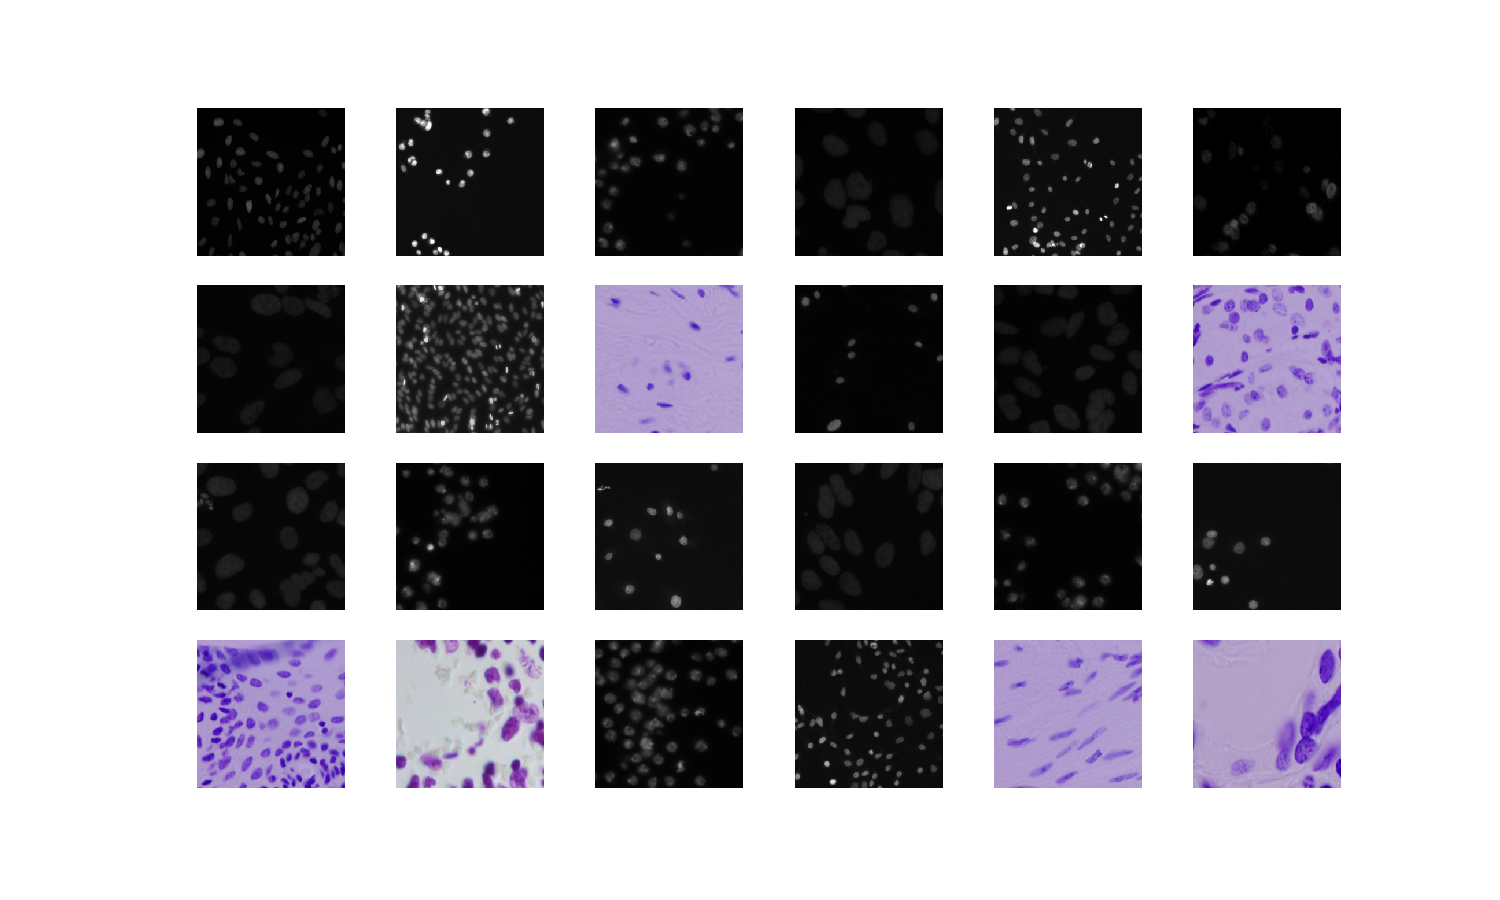
\includegraphics[width=\textwidth]{./figs/dsbowl18-imagegrid-4x6.png}
        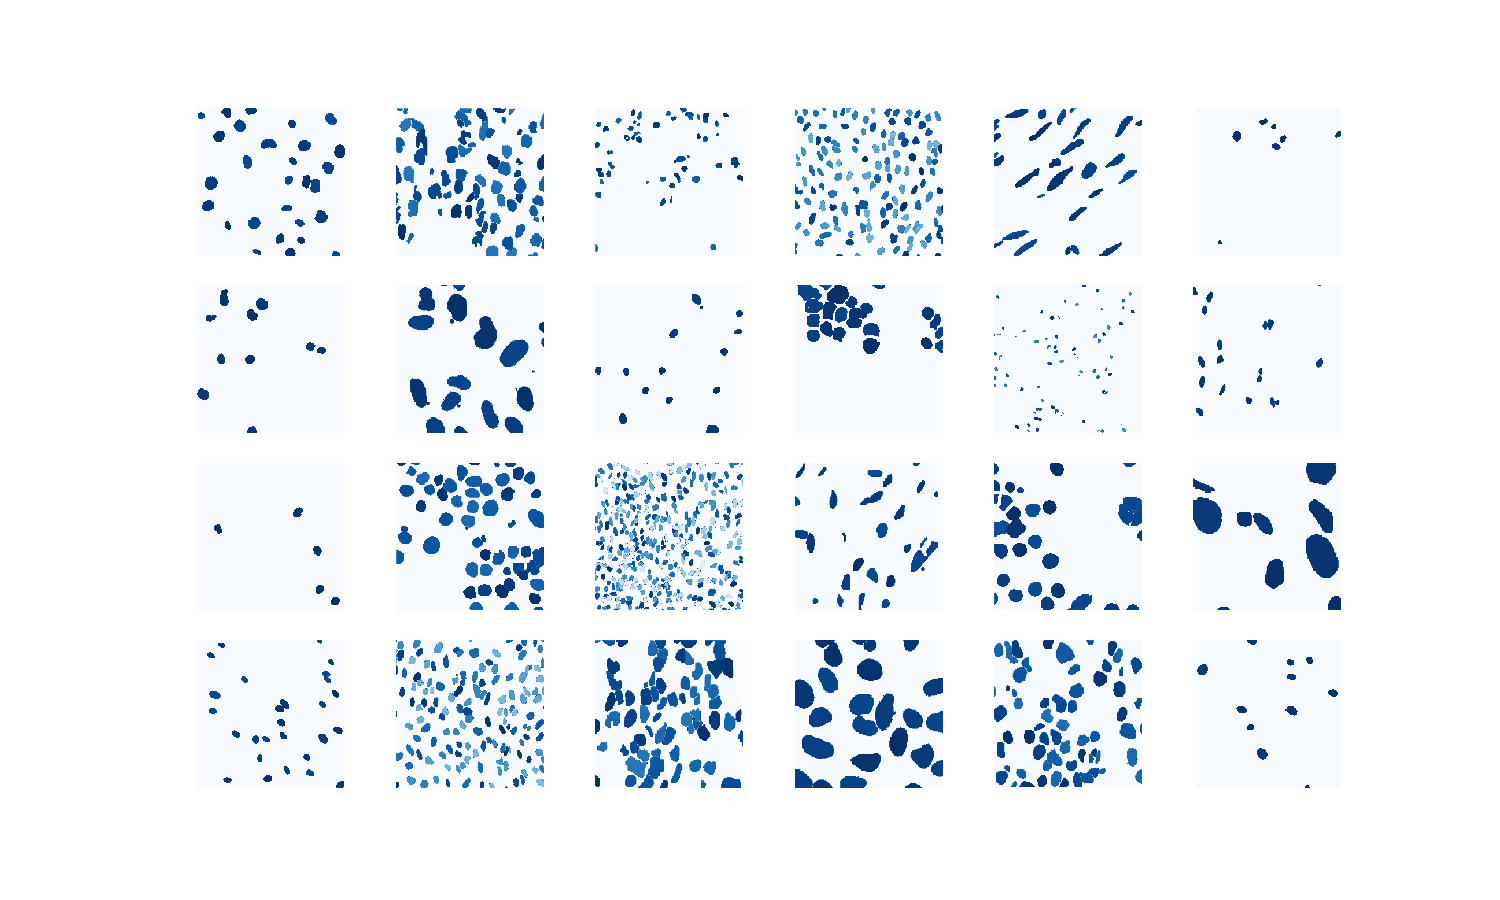
\includegraphics[width=\textwidth]{./figs/dsbowl18-imagegrid-masks-4x6.png}
        \caption{An assortment of images from our dataset.  All have been resized
        to 256 x 256. (top) raw image data (bottom) true masks }
        \label{fig:dsbowl18-grid}
    \end{figure}
\end{appendixatend}

\subsection{Formal Description of Task}

Here is a mathematical description of our task.  Given a dataset $\mathcal{D}$
composed of images, $x \in \mathbb{R}^{d}$, we'd like to learn a function $f :
\mathbb{R}^{d} \mapsto \mathbb{N}^{d}$ mapping each pixel in an input image to
a discrete nucleus label in the natural numbers.  It is key to understand that
this task is not binary classification, but rather a task of semantic
segmentation.  We wish to uniquely identify each nucleus in an image.

\subsection{Challenges}

While semantic segmentation is itself a very challenging task given any
dataset, there are some key aspects of this competition which make our task
especially challenging.
\begin{enumerate}
    \item size of training dataset

        While the recent state of the art for semantic and instance
        segmentation has been dramatically advanced in recent years, MS-COCO,
        one of the most popular datasets for such a task contains more than
        330K images, with more than 200K of them
        labeled\footnote{\href{http://cocodataset.org}{MS-COCO Dataset
        Website}}.  In contrast, our dataset contains a mere 670 labeled images
        coupled with a 67 image validation set, and a 3019 image test set.
    \item composition of dataset

        As seen in Figure \ref{fig:dsbowl18-grid}, there exist a variety of
        image types.  More specifically, the dataset was constructed using a
        number of different microscope types.  In addition, some images contain
        a rather dense assortment of nuclei while some include only a few
        sparsely distributed.
    \item mislabelings

        A significant portion of the training set has mislabeled masks.  That
        is, the reported ``true'' mask incorrectly represents the ground truth
        of the image.  Several attempts have been made by the community to
        produce better
        labels.\footnote{https://github.com/lopuhin/kaggle-dsbowl-2018-dataset-fixes}\footnote{https://github.com/ibmua/data-science-bowl-2018-train-set}
\end{enumerate}

\subsection{Metric}

Common metrics for object and semantic segmentation include average precision
(AP) at various intersection over union (IoU) thresholds, or mean average
precision (mAP) which averages the AP for each semantic class.  This
competition mostly uses AP, albeit with a somewhat modified precision
definition, detailed below.
\begin{equation}
    cP(t) = \frac{TP(t)}{TP(t) + FP(t) + FN(t)}
\end{equation}
where $cP(t)$ indicates the competition precision at $\text{IoU}=t$.  A true
positive at threshold $t$ is when we identify an object which has an IoU of at
least $t$ with a true object, false positive when a predicted object doesn't
have a corresponding true object, and a false negative if we fail to identify a
true object.  The full competition score can then be computed as
\begin{equation}
    AP = \frac{1}{10}\sum_{t = 0}^{9} cP(0.5 + 0.05t)
\end{equation}

\section{Methods}

Our pipeline consists of a few distinct steps.  We begin with aggressive
preprocessing, intended to collapse the data modalities into one.  The
processed outputs are concatenated with a set of hand-designed features
resulting in multi-channel images.  The result is a new, highly cleaned dataset
ripe for modeling.

We then pose an intermediary binary classification problem: given a pixel, does
it belong to a nucleus?  Ignoring the spatial relationship of the pixels, we
flatten our images into a large training set of individual $d$ dimensional
pixels, where $d$ is the number of channels in the original image, and the
corresponding label $y \in \{0, 1\}$ represents whether the pixel belongs to a
nucleus.  However, we frame this as a regression problem, with our outputs in
the range $[0, 1]$, so as to predict the probability of a pixel belonging to a
nucleus.  To binarize our images, we depend on a type of Deep Neural Network
(DNN) called a U-Net.

With our predicted binary mask, we proceed with the segmentation problem.  This
is accomplished using a Watershed Segmentation, with specific care to perform
non-maximum supression on the proposed markers so as to limit oversegmentation.

\subsection{Preprocessing \& Data Whitening}

Acknowledging that the data is composed of several modalities, our first step
is to effectively preprocess our images into a single unimodal distribution.
Our approach can be broken into 3 steps:
\begin{enumerate}
    \item reshape \& rescale pixel values to $[0, 1]$
    \item invert images with a white background and dark nuclei
    \item transfer a desired color distribution onto all images by whitening
\end{enumerate}

The first step, reshaping and scaling is somewhat self-explanatory.  We require
that all images are of one size for a few reasons.  Firstly, it greatly
simplifies implementation and speeds up computation, as it allows us to use
fixed-size arrays $n$-dimensional arrays rather than using a slower dynamic
data structure.  It also affects scale-dependent hyperparameters.  If we use a
range of image sizes, then the best hyperparameters might be different for each
size class, increasing the number we must choose.

We follow this by an inversion of all images with a white background.  In
images with white backgrounds, the nuclei are dark, while in images with a
black or dark background, the nuclei are white or light.  Naively training a
classifier on the raw data can result in examples which contribute conflicting
information to our loss landscape.  To rectify this, we simply invert images
with a white background, so that the background becomes dark and the nuclei
become light.  The binary classification problem between background and nuclei
becomes less a problem of local structure in an image and more one of
the individual pixel content compared to neighbors.

Over the past few months and years, there's been a rise in publications
involving neural style transfer, many of which who employ deep neural networks
to transfer the style of one image to the content of another. We initially
tried this approach, attempting to transfer the dark background and light
nuclei style of several of the training images to some of the more difficult
training images with lighter back grounds. Unfortunately, in practice this
proved be to be far too resource demanding and time consuming.

However, applying neural style transfer to this problem is a \textbf{sin of
overengineering}. Note that the color of an image is simply defined as the
ratio of the red green and blue color channels of an image.  We approach this
problem as a problem of finding the right basis space with which to represent
our data.  Assuming that our data naturally exists in a latent space with
unknown basis vectors, we posit that we can return our data to this space
through simple linear transformations, completely unsupervised.  Given a
flattened $d$-channel image with $n$ pixels, $X_j \in \mathbb{R}^{n \times d}$,
we propose that its content was colored according to the simple matrix
equation
\begin{equation}
    X_j = S_j X^*_j
\end{equation}

where $S_j$ is the coloring matrix, and $X^*_j$ is our original content in the
latent space.  Of course, provided $S_j$ is an invertible matrix, we can
succeed in full recovery of our data.  However, we must be careful to transform
each image to the \textit{same} latent space.  Of course, we're not the first
to do this.\cite{whiten-stanford}\cite{whiten-mit}  This practice is known as
whitening the data, in which we uncorrelate the features.  As seen in Figure
\ref{fig:correlated-features}, the channels in our raw images are highly
correlated.  Since we'd prefer our images (at least in this initial first pixel
classification model) to be greyscale, with as much variance as possible, this
problem becomes incredibly tractable.  Our task reduces to decorrelating the
images channels (recovering our latent space), and taking the channel
corresponding to the highest variance.  This is accomplished using PCA
whitening.

\begin{figure}
    \centering
    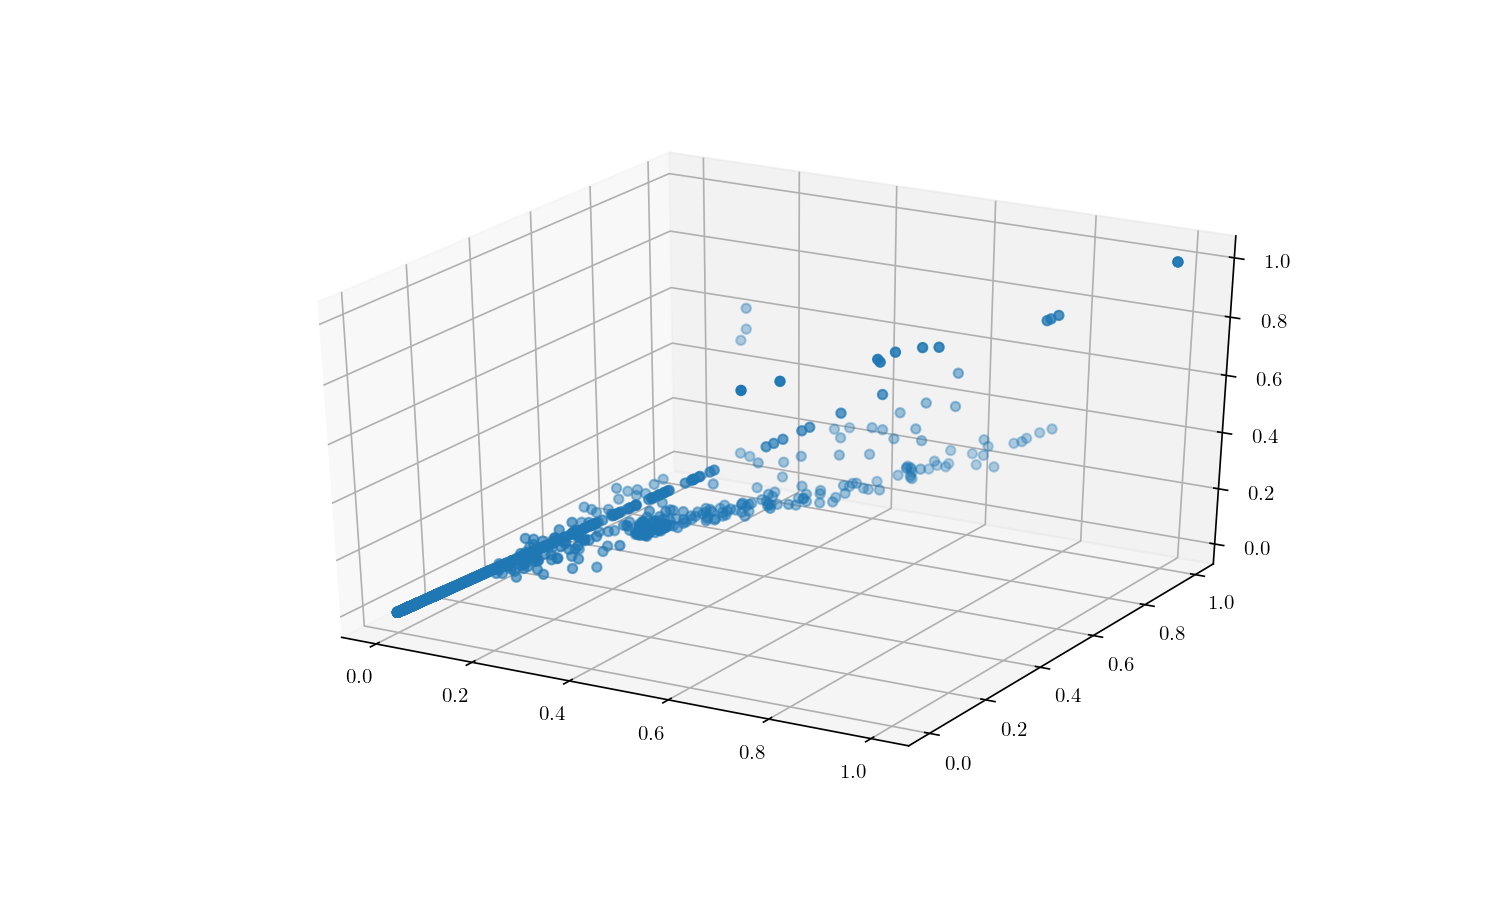
\includegraphics[width=0.75\textwidth]{./figs/correlated-features.png}
    \caption{A scatter plot of a subset of pixels from our training data.
    Notice how clear lines form, representing various modalities, all with
    highly correlated features.}
    \label{fig:correlated-features}
\end{figure}

\subsection{Hand Designed Features}

After whitening the data, we mapped our data into a feature-space with goals of
extracting as much information as possible and creating as much contrast between
foreground and background as possible.

We came accross these features by extracting over 10 features that could encode
further information, fitting the regressors, and then checking the regressors'
weight vectors to see if each feature was important. After performing this
process several times, we ended up with 5 features. Below, we describe the
information each feature encodes and the intuition behind including that information:

\begin{enumerate}
  \item Raw RGB Values:
  We first decided the include the RGB values themselves. Several other
  existing pipelines relied solely on the RGB values and performed quite well,
  meaning the RGB values must encode valuable information, so we included them.
  \item  Bilateral Filter:
  A Bilateral Filter convolves the image with a weighted Gaussian kernal. This
  denoises the image, while still preserving the edges. We included it to
  get rid of background salt and pepper.
  \item 50/99 Image Rescaling:
  Image Rescaling widens the data distribution and increases contrast. We grabbed
  the 50th percentile and rescaled everything below and including that value to
  be 0, and we grabbed the 99th percentile and rescaled everything above that
  value to be 1. We included this to increase contrast between foreground and background,
  and to filter out salt and pepper.
  \item Adaptive Histogram Equalization:
  Adaptive Histogram equalization increases contrast locally. We included this
  so that the regressors could recognize smaller nuclei among salt and papper.
  \item Dilation:
  A dilation performs a uniform kernel convolution accross the image, thus
  setting each pixel to be the average of its neighbors and itself. This increases
  the area of each nucleus. We included this so that the regressors could pick
  out small nuclei.

\end{enumerate}
After extracting these feature, we perform standard feature normalization on
each feature.



\subsection{Linear Model for Individual Pixel Probabilities}

This stage of our pipeline is tasked with taking an input vector $x \in
\mathbb{R}^d$ and assigning to it a probability of belonging to a nucleus.
Mathematically, we wish to learn a function $f: \mathbb{R}^d \mapsto [0, 1]$
which minimizes the binary cross-entropy loss
\begin{equation}
    \mathcal{L}(\mathcal{D}) =
        - \sum_{x \in \mathcal{D}} yf(x) + (1 - y)(1 - f(x))
\end{equation}

While we discussed several techniques for performing soft-classification, the
largest factor of consideration for us is computational tractability.  While
our training dataset is rather small in terms of individual
images\footnote{Dataset Sizes: Training (670), Validation (65), Testing
(3036)}, after decomposing these sets into pixels our dataset becomes quite
large.  In our implementation we resized all images to $256 \times 256$, which
results in a 65536x increase in the number of training examples.  One
trick to reduce this, due to the sparsity of many training examples and the
over-abundance of negative examples, is to simply filter out some of the number
of negative examples.  In practice, training on the entire dataset limits us to
algorithms using some form of stochastic gradient descent (SGD), as it's
infeasible to perform matrix operations to calculate an exact least squares
solution on the full dataset.

We use two regression models in our model pipeline, both implemented in
Scikit-Learn\cite{scikit-learn}: the \texttt{SGDRegressor} and the
\texttt{PassiveAggressiveRegressor}\cite{paregression}.  These models were
chosen as they are fast, tested, and available implementations for linear
regression.  In practice, the two models focused on different subsets of our
features mentioned above, and their learned outputs have considerable variance.
We chose to include both as it improved our individual pixel classification
precision and recall.

We'll continue by explaining in detail the mathematical problems each of these
implementations solve as well as the hyperparameters involved.

\subsubsection{\texttt{SGDRegressor}}

This regressor solves linear regression using the standard squared loss, so as
to approximate the Ordinary Least Squares (OLS) solution to the system of
equations.  Regularization is induced by an elastic net with a mixing
coefficient to combine $\ell_1$ and $\ell_2$ regularization.
\begin{equation*}
    \hat{\theta} = \argmin_\theta
        \left\{ \sum_{x \in \mathcal{D}} (y - \langle \theta, x \rangle)^2
                + \alpha\left(
                    \gamma\abs{\theta}_1 + (1 - \gamma)\abs{\theta}^2_2
                  \right)
        \right\}
\end{equation*}

where $\gamma$ is our mixing coefficient, and $\alpha$ is our regularization
term.

\subsubsection{\texttt{PassiveAggressiveRegressor}}

This regressor has roots in standard linear regression as well as Support
Vector Machines (SVM).\cite{paregression}  It tackles standard binary classification
as well as regression, however it's weight update is quite unique.  At step
$t$, the new weight vector $w_{t+1}$ is defined as
\begin{equation*}
    w_{t+1} = \argmin_{w \in \mathbb{R}^n} \frac{1}{2}\abs{w - w_t}^2
\end{equation*}

such that $\ell(w; (x_t, y_t)) = 0$, where $\ell$ represents the hinge loss at
step $t$.  Let's explore what happens for a given $w$.  Suppose that the hinge
loss is already 0.  Then the algorithm is completely \textit{passive}, as it
simply chooses $w_{t+1} = w$.  Else, we \textit{aggressively} force $w_t$
to satisfy $\ell_t$ by projecting in onto the space of vectors such that
$\ell_t = 0$.

In practice, much like fitting an SVM, we introduce a slack variable to control
the \textit{aggressiveness} of the regressor, as seen below.
\begin{equation*}
    w_{t+1} = \argmin_{w \in \mathbb{R}^n} \frac{1}{2}\abs{w - w_t}^2 + C\xi
\end{equation*}

such that $\ell(w; (x_t, y_t)) \le \xi$ and $\xi \ge 0$.

\subsection{U-Net as a Learned Binarizer}

Stacking our predictions from our linear models with our 5 features, we complete
our pipeline using a DNN functioning as a learned binarizer called a ``U-Net"
\footnote{\href{https://arxiv.org/pdf/1505.04597.pdf}{The Original U-Net Proposition Paper}}.
The goal of the U-Net is to segment the image. That is, the U-Net learns a function
$f : \mathbb{R} \mapsto \{0, 1\}$ for each pixel such that a class label is assigned
to each pixel. For the purpose of our pipeline, the classes are
\begin{enumerate}
  \item $0$ if we predict a pixel is not part of a nucleus
  \item $1$ if we predict a pixel is part of a nucleus
\end{enumerate}

\subsubsection{General U-Net Architecture}
To segment the image, a U-Net ``supplement[s] a usual contracting network by
successive layers, where pooling operators are replaced by upsampling
operators. In order to localize, high resolution features from the contracting
path are combined with the upsampled output" (Ronneberger et al. 2). Stacking
the high-resolution features with the unsampled output results in symmetry
between the expansive path and the contracting path, resulting in a u-shape as
seen in Figure \ref{fig:U-Net-architecture}. For the image borders, U-Net
extrapolates missing information by mirroring the original image accross the
image borders.

\subsubsection{Our U-Net Architecture}
Our U-Net Architecture is very similar to the original U-Net Architecture. The
only modification we made was in the image dimensions. Rather than starting at
a 572x572 resolution and pooling down to 32x32 images at the lowest
resolution, we start at a 256x256 resolution and pool down to a 32x32 image,
halfing each image dimension with all 3 pooling layers. Other that this
modification, our architecture is exactly that described in
\href{https://arxiv.org/pdf/1505.04597.pdf}{The Original U-Net Proposition
Paper}.  The Keras code to describe the first iteration of our U-Net
architecture was taken from a
\href{https://www.kaggle.com/toregil/a-lung-u-net-in-keras}{Kaggle Kernel for
CT Lung Data}.

\subsubsection{Why This Architecture?}
We attempted several other network architectures. Most notably, we tried
VGG-segnet and Keras-FCN, finding that our U-Net resulted in the highest
pixel-F1 score. Furthermore, we attempted deeper U-Nets, finding that further
levels of abstraction did not provide significant pixel-wise F1 improvement
after 50 epochs. We also attempted more shallow U-Nets, finding that
decreasing the number of layers lowered our pixel-wise F1 score a significant
amount after 50 epochs.

\subsubsection{ Data Augmentation }
As prior mentioned, we only had 670 training images and 67 validation images provided by Kaggle.
Thus, to create more data, we used a Keras data augmentation generator to "create" more data
and control overfitting. In the data augmentation generator, we allowed for horizontal and
vertical flipping, zooming, as well as shearing. We fed this data generator into the U-Net, which
improved our validation pixel F1 score from $.85$ to $.89$.

\begin{appendixatend}
    \subsection{U-Net Architecture}
    \begin{figure}
        \centering
        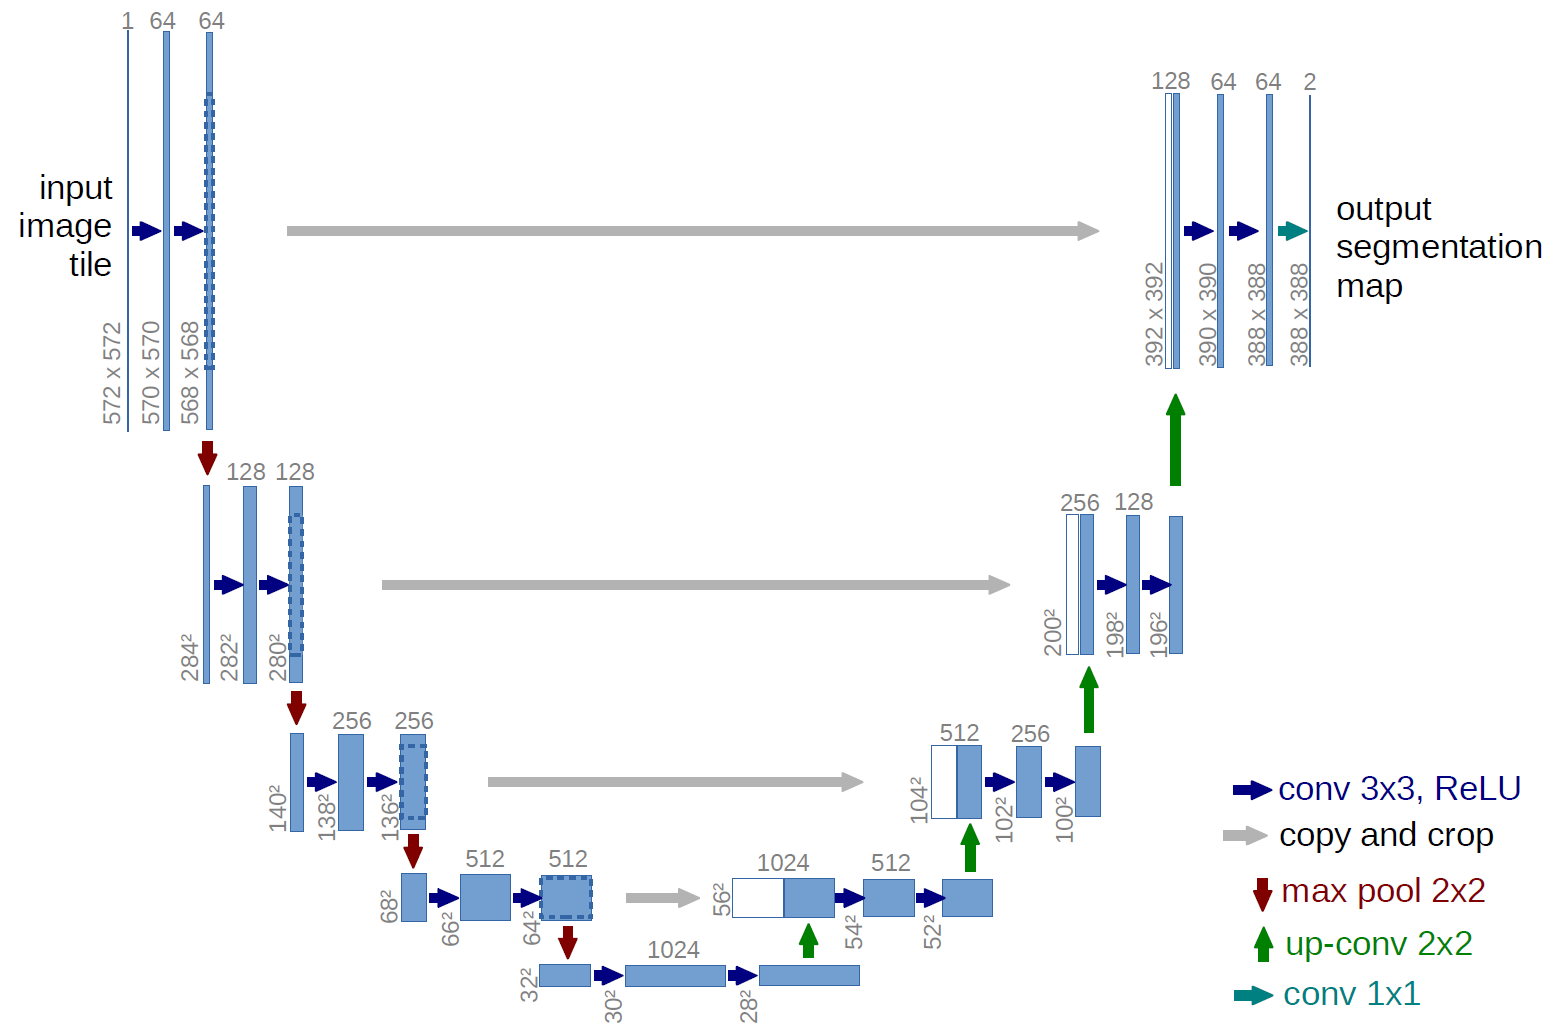
\includegraphics[width=\textwidth]{./figs/unet_architecture.png}
        \caption{The U-Net Architecture, as presented in  \href{https://arxiv.org/pdf/1505.04597.pdf}{The Original U-Net Proposition Paper} }
        \label{fig:U-Net-architecture}
    \end{figure}
\end{appendixatend}

\subsection{Semantic Segmentation using Watershed}

At this point in our pipeline, we have binary masks for each nuclei image.
From here, we need to develop individual masks for each nucleus in an image.
To accomplish this, we use the watershed algorithm to help us segment each
nucleus.  Given a binary mask, we perform this process to segment our nuclei:
\begin{enumerate}
    \item perform a euclidean distance transform

        The distance transform calculates the distance to the nearest 0 value
        in $\ell_2$ pixel distances.  This has the effect of producing high
        transform values for pixels in the center of a nucleus.

    \item local max calculation and non-maximum supression

        With the distance transform, we find the local maxes to identify
        potential nuclei centers.  To prevent oversegmentation, we filter our
        set of local maxes to limit the number in a given region, or if we
        detect that two are part of the same nucleus.

    \item watershed segmentation using the distance transform, with the local
        maxes as basin markers

        The watershed segmentation works by taking samples of a signal (our
        distance transform), as well as markers (our local maxes), and begins
        filling ``basins'' in the signal at the markers.  In practice, we use
        the negative of the distance transform.  The edges of a cluster in the
        segmentation are when the basin spills over to the ``surface''.
\end{enumerate}

The segmentation sounds perfect in theory, but struggles with oversegmentation
in practice due to the local max calculation.  We attempt to handle the local
max filtering with some simple heuristics, but we could get more advanced with
how we decide to keep or reject a local max.

\section{Results}

\subsection{Preprocessing \& Data Whitening}

After applying our preprocessing steps, we result in high-quality grayscale
images.  A comparison between raw modalities and our processed images is
presented in Figure \ref{fig:processing-results}.  In our PCA projection,
we consistently explain 97\% of the original channel variance in the first
principal component of our data.

\begin{figure}[H]
    \centering
    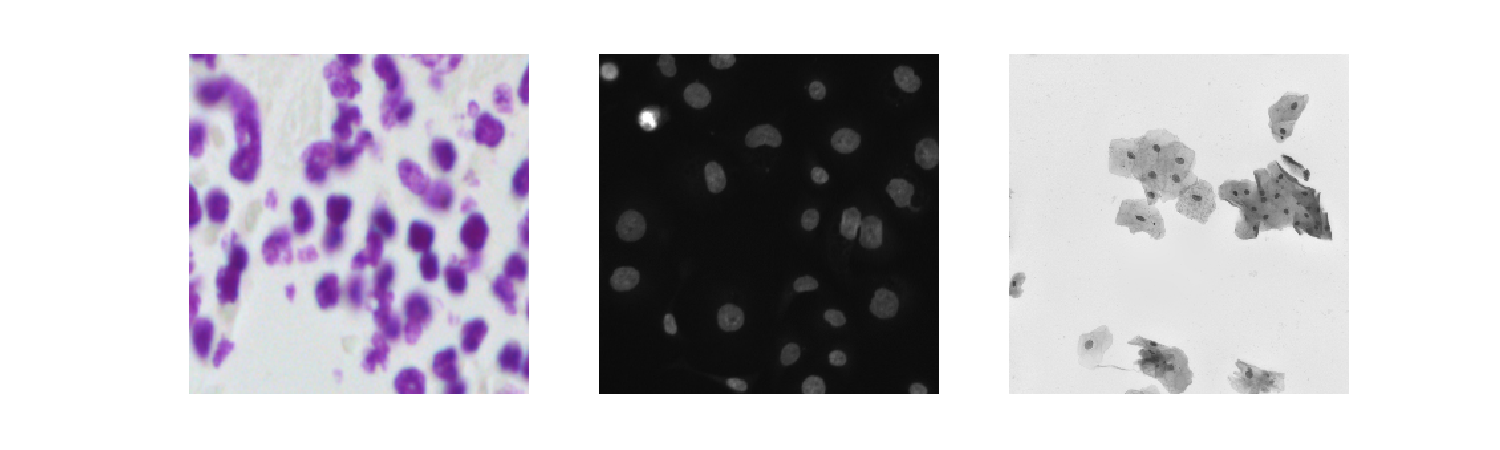
\includegraphics[width=0.85\textwidth]{./figs/raw-modalities.png}
    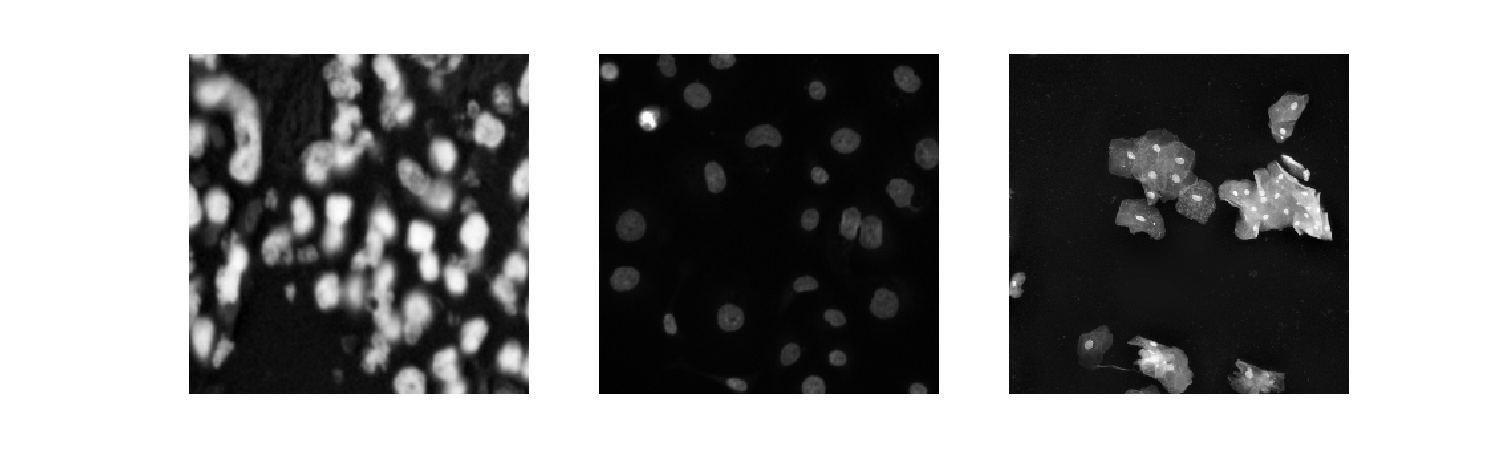
\includegraphics[width=0.85\textwidth]{./figs/processed-modalities.png}
    \caption{Comparison between the raw images (top) and our processing steps
    (bottom).}
    \label{fig:processing-results}
\end{figure}

\subsection{Hand Designed Features}

\begin{figure}[H]
    \centering
    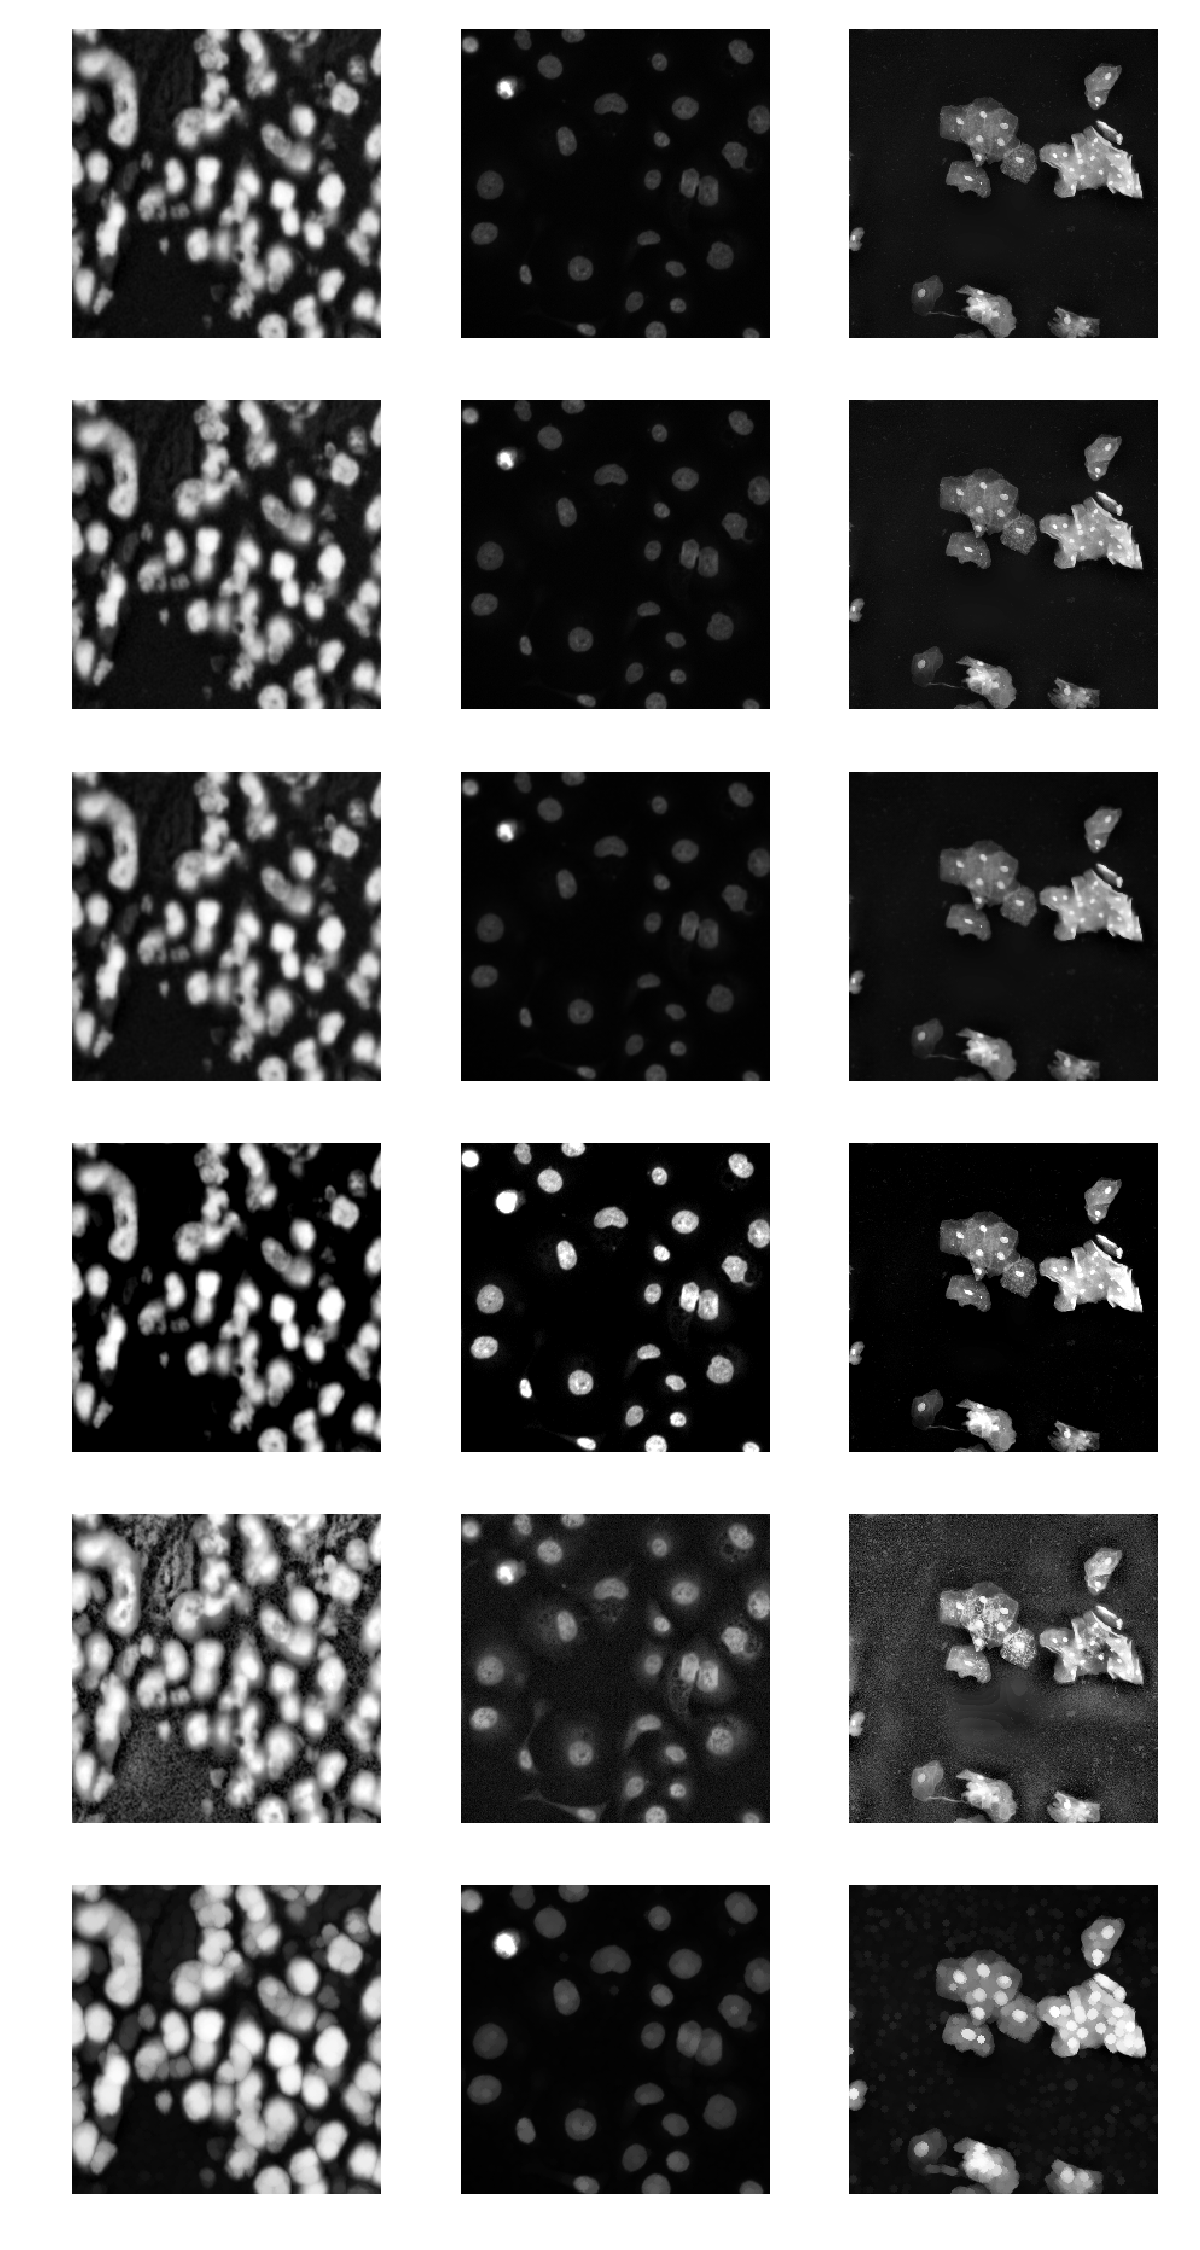
\includegraphics[width=0.65\textwidth]{./figs/hand-designed-features.png}
    \caption{Our feature transforms applied to 3 different image modalities.  The
    features are listed vertically in the following order: (1) preprocessed (2)
    z-score (3) bilateral filtering (4) rescaled image (5) histogram
    equalization (6) dilation.}
    \label{fig:hand-designed-comparison}
\end{figure}

Our feature representation for each modality can be seen in Figure
\ref{fig:hand-designed-comparison}.

\subsection{Linear Model for Individual Pixel Probabilities}

\subsection{U-Net as a Learned Binarizer}

\subsection{Semantic Segmentation using Watershed}

\section{Discussion}

\subsection{ Dataset Insights }
Our various experiments revealed that the data is much noiser than we thought.
We thought that feeding the U-Net as much information as possible would allow
the U-Net to model this background noise. However, we believe that the distribution
of noise is different depending on the data modality, and was thus difficult for the
U-Net to learn. Thus, we also learned that although DNN's are excellent at
providing abstract representations of the data, they cannot learn multiple noise
distributions given such a small dataset. To fix this problem, we would've liked to
preprocess the data in a way such that all modalities are unified in both foreground
and background noise, or to use unsupervised learning to cluster the data based on
their underlying distribution and to then predict each new image based on a process
specialized to its underlying distribution.

\subsection{ Pipeline Selection }

We ultimately developed two pipelines: the pipeline described above, and a Mask RCNN
based off of the \href{Matterport Implementation}{https://github.com/matterport/Mask\_RCNN}.
For the Mask RCNN, we simply modified the code to train on the provided nucleus training set
and to give predictions for the stage 1 test set. After doing so, we recieved an AP score of
$.477$ \footnote{This score of .477 is based off of our local implementation of AP using the
Stage 1 data for scoring.}. However, we felt as if the purpose of the project is to
learn about machine learning, and we did not believe that we learned much by using
someone else's implementation of an architecture we did not fully understand.
So, even though Mask RCNN outperformed our pipeline described above, we did not
consider the Mask RCNN our work, nor did we believe that it taught us much of
anything. Hence our rationale for ultimately submitting the pipeline described
above.

As for how we went about selecting the specific steps in our pipeline, we thoughts
of this problem as two-stage: predicting if a pixel is part of a nucleus
(i.e. binarization), then predicting which pixel it is part of (i.e. segmentation).
For the binarization step, we saw that U-Net was successful, so we decided to feed
in as much information as possible to our U-Net. For segmentation, watershed seemed
reasonable, but also oversegmented very frequently, so we modified it to include a
non-maximum suppression step. To unify the modalities, we preprocessed the data by
whitening. And to get rid of holes in the image, we performed a
\texttt{$binary\_fill\_holes$} operation.

\subsection{ Lessons on Large-Scale Prediction Problems }

We learned several lesson from this project:

\begin{enumerate}
  \item In a pipeline, each step needs to perform well. It is very difficult to
  make up for a bad stage in a pipeline, and it is very important to identify
  which stages perform poorly and to spend time and effort improving those stages.
  \item Implementing an evaluation metric for the entire pipeline early on is
  extremely important. We had two major stages in our pipeline: binarization
  and segmentation. We knew that the binarization step performed very well from
  validation pixel F1 scores. From qualitative assessment, we assumed that the
  segmentation step was performing well. However, when we finally implemented a
  submission method that allowed us to evaluate our pipeline, we learned that it
  did not perform nearly as well as expected. Via process of elimination, we
  learned that it was the segmentation step in our pipeline that was performing
  poorly, but only after it was too late to try anything radically new.
  \item On a related note, every stage in a pipeline should be evaluated
  quantitatively, not just qualitatively
\end{enumerate}


\section{Conclusion}

\newpage

\printbibliography

\newpage

\includeappendices

\end{document}
